\documentclass[12pt]{article}
\usepackage{amsmath}
\usepackage{mathtools}
\usepackage{bigints}
\usepackage{parskip}
\usepackage{amssymb}
\usepackage{relsize}
\usepackage{fullpage}
% \DeclareMathSizes{12}{17.28}{9}{7} % (a)

\DeclareMathSizes{12}{17.28}{12}{12} % (a)


\usepackage{hyperref}



	\addtolength{\topmargin}{-.5in}
	\addtolength{\textheight}{1.75in}



    \newenvironment{myindentpar}[1]%
     {\begin{list}{}%
             {\setlength{\leftmargin}{#1}}%
             \item[]%
     }
     {\end{list}}

\begin{document}
\title{College Algebra: Module 7 What You Need To Know}
\date{2-26-15}
\author{}
\maketitle


\section{Linear Graphs and Rates of Change (Section 2.2)}

\textbf{Linear Equation} - a \textit{linear equation} is any equation that can be written in the form
\newline

\centerline{$ax + by = c$}

where $a,b,c$ are real numbers 

{\bf \underline{Intercepts}}
\begin{myindentpar}{1cm}
\textbf{Y-intercept} - the point where a graph passes through the y-axis. To find the y-intercept we set $x=0$ and solve for $y$

\textbf{X-intercept} - the point where a graph passes through the x-axis. To find the x-intercept we set $y=0$ and solve for $x$
\end{myindentpar}

{\bf \underline{Lines:}}
\begin{myindentpar}{1cm}
\textbf{Slope of a Line: } Given two different points $(x_{1},y_{1})$ and $(x_{2}, y_{2})$ the \textit{slope} of the line connecting these two points is given by
\newline

\centerline{$m = \dfrac{y_{2} - y_{1}}{x_{2}-x_{1}}$}
\vspace{.5cm}

\textbf{Parallel Lines:} two lines are parallel if they have the same slope
\vspace{.5cm}

\textbf{Perpendicular Lines:} two lines are perpendicular if the slope of one line is the \textbf{negative reciprocal} of the slope of the other line

\vspace{.5cm}

\textbf{Horizontal Lines:} the equation of a horizontal line is given by
\newline

\centerline{$y = k$} 

where $k$ is some real number. The \textbf{slope of a horizontal line is always 0.}

\vspace{.5cm}

\textbf{Vertical Lines:} the equation of a vertical line is given by
\newline

\centerline{$x = h$} 

where $h$ is some real number. The \textbf{slope of a vertical line is always undefined.}
\end{myindentpar}

\vspace{.5cm}

\underline{\textbf{Positive, Negative, Zero, or Undefined Slope:}}

\centerline{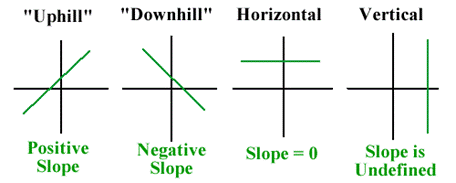
\includegraphics{Slope.png}}

\section{Graphs and Special Forms of Linear Equations (Section 2.3)}

\textbf{Point-Slope Equation of a Line:} The line with slope $m$ passing through $(x_{1}, y_{1})$ is given by
\newline

\centerline{$y - y_{1} = m(x-x_{1})$}
\vspace{.5cm}

\textbf{Slope Intercept Equation of a Line:} The line with slope $m$ has a slope-intercept form of 
\newline

\centerline{$y = mx+b$ \hspace{1cm} where (0,b) is the y-intercept}
\vspace{.5cm}

\newpage

\textbf{Word Problem 1}

\centerline{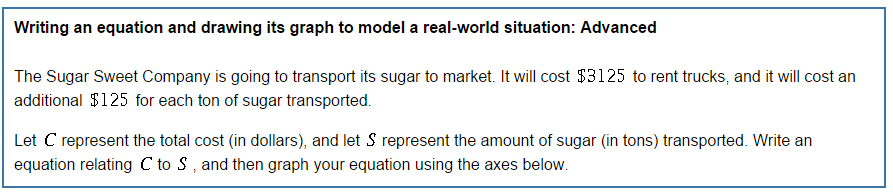
\includegraphics[scale = 0.9]{WordProblem1.png}}

\newpage

\textbf{Word Problem 2}

\centerline{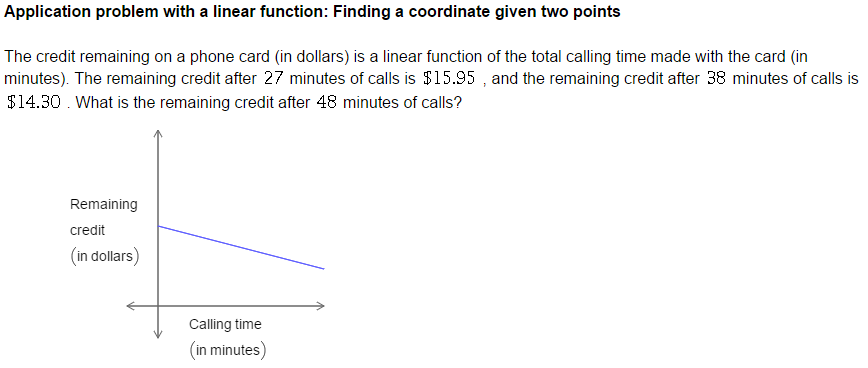
\includegraphics[scale = 0.9]{WordProblem2.png}}










\end{document}